\chapter{Optical techniques for brain activity measurements}
\label{ch:detectors}
The best method for measuring brain temperature is to use a thermocouple probe placed in direct contact with the tissue.  Experimental measurements of brain temperature have achieved a precision as small as $0.000\,3$\degree C using this method~\citep{mcelligott}. However, this method can not be used in humans without damaging the tissue.  An optical method would be ideal for non-invasive measurements.  Presently, there does not exist a method for accurately measuring the temperature of brain tissues optically.  However, other optical measurements methods could be used in conjunction with a temperature model (such as the one proposed here) to calculate the temperature.  The possible application of functional Near-Infrared Spectroscopy (fNIRS) and its possible use in brain temperature calculations is discussed along with the possibilities and limitations of a direct measurement technique such as thermal imaging.
  
\section{{F}unctional {N}ear-{I}nfrared {fNIR} Spectroscopy}
% detector applicaitons to improving fNIR
\begin{figure}[tb]
  \begin{center}
    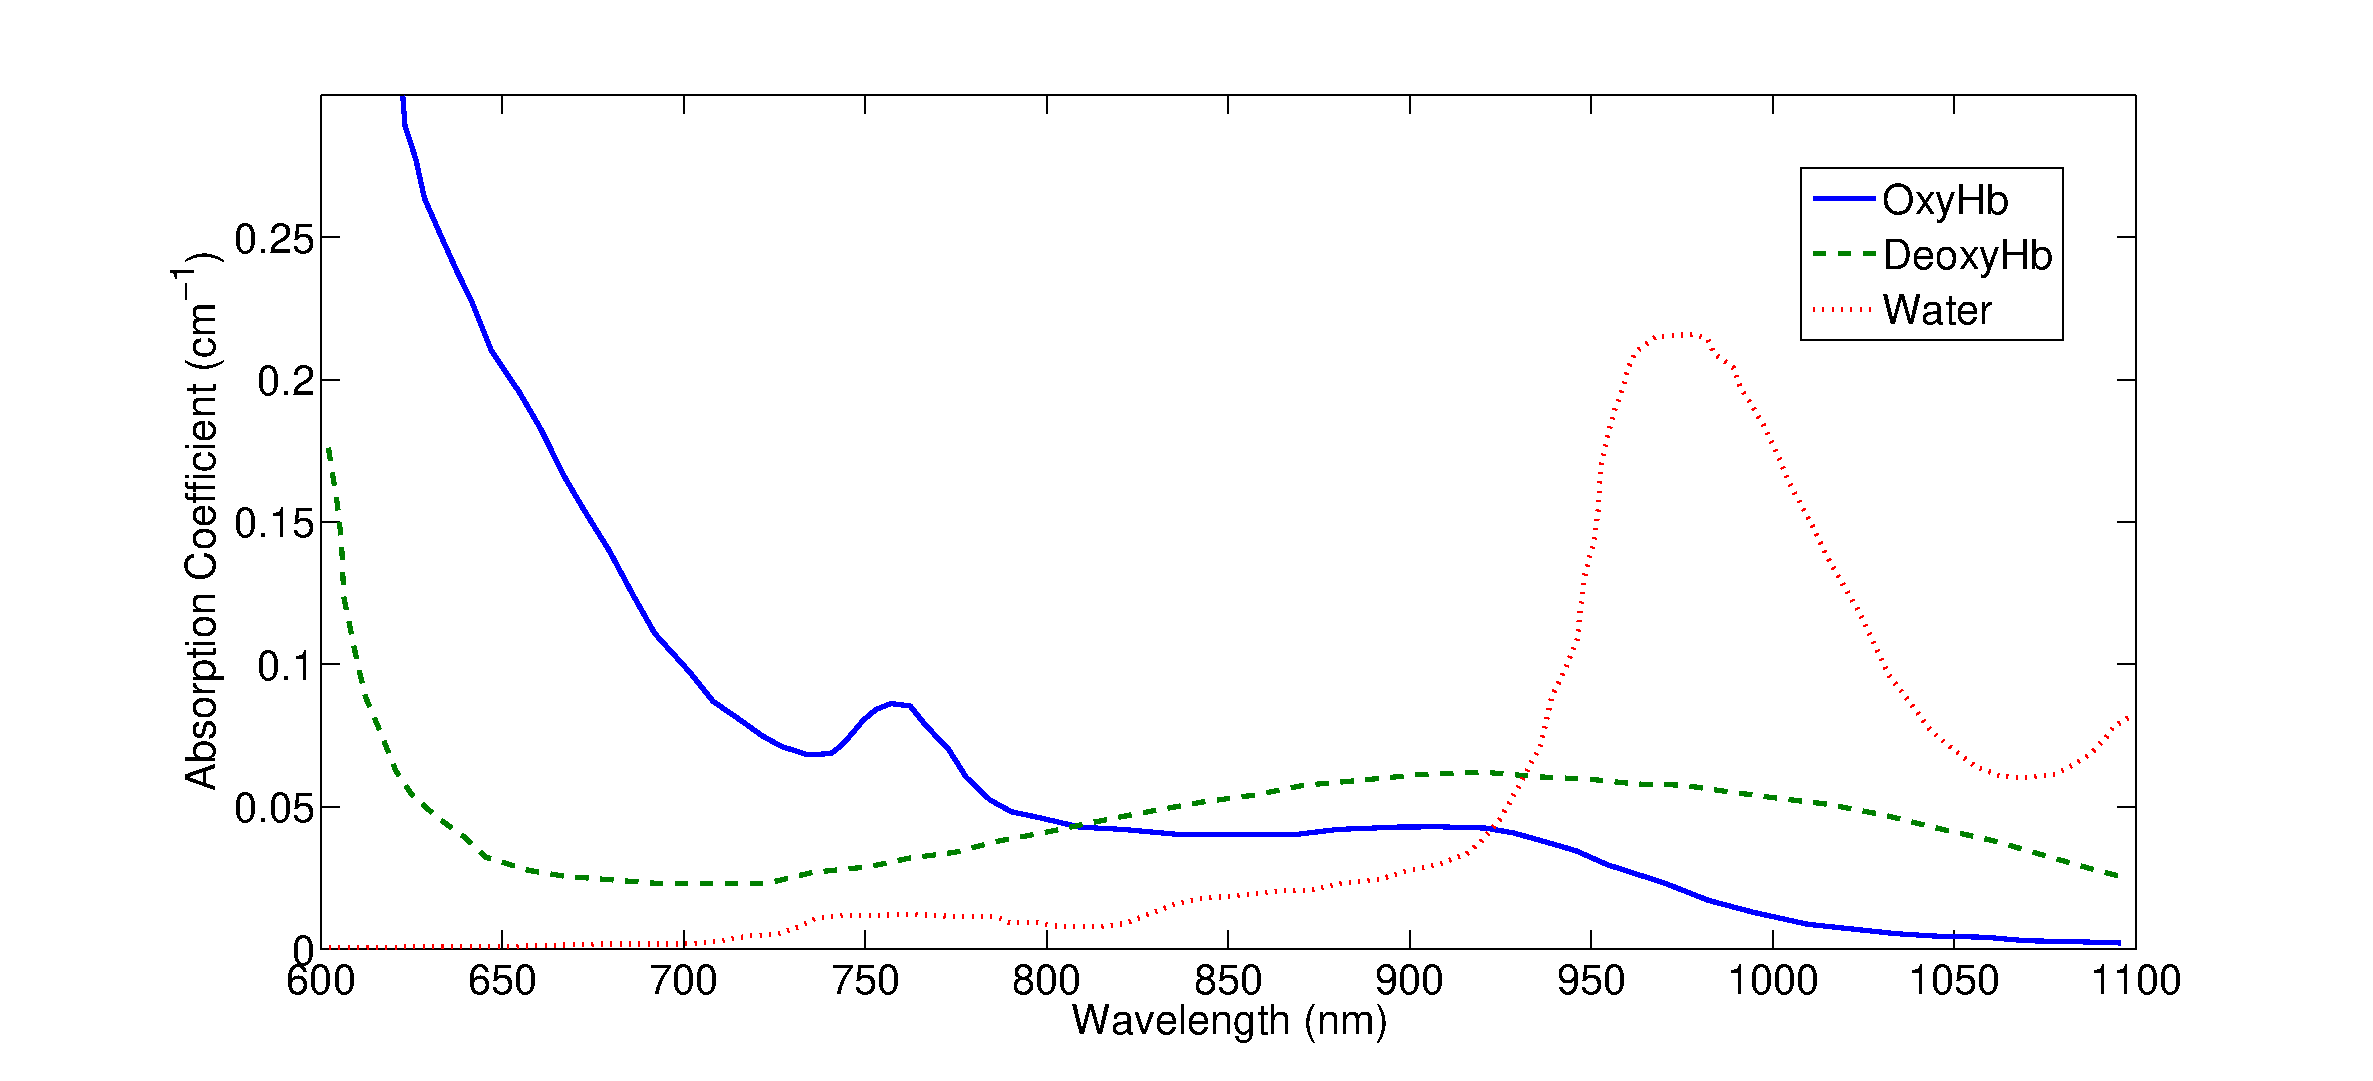
\includegraphics{AbsorptionData}
    \caption[Absorption spectra of water, deoxyhemoglobin and oxyhemoblogin]{\label{fig:fnirabsorption} Absorption spectra of water~\citet{cope}, oxyHb and deoxyHb~\citet{horecker}.}
  \end{center}
\end{figure}
\begin{table*}[tb]
  \begin{tabular*}{\linewidth}{lp{5cm}p{5cm}}
    \toprule
                         & fMRI             & fNIR            \\
    \midrule
    Spatial Resolution   & 8--27 mm$^3$  & $\sim$ 1--10 cm$^3$ \\
    Temporal Resolution  & 1--2 s        & $\sim$ 10$^{-3}$ s \\
    Measurement Parameter& blood volume, flow, and O$_2$ metabolism & oxyHb and deoxyHb concentrations \\
    Motion               & Must Remain Stationary & Small movements OK \\
    Penetration          & Whole-head    & outer 2--4 mm of brain tissue \\
    \bottomrule
  \end{tabular*}
  \caption[Comparison of fMRI and fNIR]{\label{tbl:comaparemethods}Comparison of the capabilities and limitations of fMRI and fNIR techniques.  Compiled from~\citet{bunce2006,elliott}.}
\end{table*}

As discussed in~\cref{ch:introduction}, changes in tissue activity can be detected by measuring the change in blood oxygenation levels.  Functional Magnetic Resonance Imaging (fMRI) is one technique among several for measuring tissue oxygenation (the BOLD signal).

Blood oxygenation can be determined by measuring the relative concentrations of oxyhemoglobin (oxyHb) and deoxyhemoglobin (deoxyHb)~\citep{ogawa1990,kwong1992,fox1986}.  Since oxyHb and deoxyHb have different absorption spectra as shown in~\cref{fig:fnirabsorption}. These differences are possible to detect  through optical techniques.  Functional Near-Infrared Spectroscopy is a technique which utilizes two or more spectral bands in order to determine blood oxygenation.  fNIRS has a high (millisecond) temporal resolution and a low ($\sim$1~cm$^3$) spatial resolution compared to fMRI (as low as 1 mm$^3$). Also, fNIRS is limited to only imaging the outer cortex (2--4~mm)~\citep{bunce2006}. A comparison of fMRI and fNIR is presented in~\cref{tbl:comaparemethods}.

fNIRS works by utilizing an array of near-infrared detectors and emitters (typically spaced 2--3~cm apart) placed in contact with the skin~\citep{villringer1997,izzetoglu2004}.  A schematic of a typical fNIRS array setup is shown in~\cref{fig:fnir-arragement}. Each dashed line is a detection path. By illuminating the emitters sequentially, it is possible to have 16 detection channels using the setup shown.  The exact spacing between the emitters and detectors determines the depth the light is detected from.  As shown in~\cref{fig:fnirpenetration}, the closer the spacing, the higher the resolution but at the expense of lower penetration.  Conversely, in order to detect light passing through deeper tissue, a wider spacing is used which reduces the resolution.  Systems use either two~\citep{villringer1997,izzetoglu2004p,sato2004} or three~\citep{hoshi2003} wavelengths selected based on differences in the absorption of oxyHb and deoxyHb.  The exact wavelengths used vary, but all lie within an optical window between 700--1000~nm~\citep{villringer1997} where the near-infrared photon absorption in the tissue is low~(\cref{fig:fnirabsorption}).

\begin{figure}[tb]
  \centering
  \tikzstyle{detector} = [circle,draw, ultra thick, fill=blue!20]
\tikzstyle{ann} = [draw=none,fill=none,right]
\tikzstyle{led} = [star,star points=10,draw, thick, fill=red]
\tikzstyle{l} = [draw, very thick, color=black, dashed]
\tikzstyle{legend-box} = [rectangle, draw, thick, fill=none, minimum height=2cm, minimum width=3.5cm]
\begin{tikzpicture}
  \matrix[row sep=1cm,column sep=1cm] {
  \node[detector] (d11) {}; & &
  \node[detector] (d12) {}; & &
  \node[detector] (d13) {}; & &
  \node[detector] (d14) {}; & &
  \node[detector] (d15) {}; \\
  & \node[led] (e1) {}; &
  & \node[led] (e2) {}; &
  & \node[led] (e3) {}; &
  & \node[led] (e4) {}; \\
  \node[detector] (d21) {}; & &
  \node[detector] (d22) {}; & &
  \node[detector] (d23) {}; & &
  \node[detector] (d24) {}; & &
  \node[detector] (d25) {};\\
  };
  \node[ann, right=of d11, yshift=-0.6cm, xshift=-0.3cm] {L};
  \node[detector, right=of d15, yshift=-1.2cm] (dRef) {};
  \node[led, below=of dRef, yshift=0.7cm]      (eRef) {};
  \node[ann, right=of dRef, xshift=-0.9cm] {Detector};
  \node[ann, right=of eRef, xshift=-0.9cm] {Emitter};
  \node[legend-box, below=of dRef, yshift=1.8cm, xshift=1cm]{};
  \path[l](d11.south east) -- (e1.north west);
  \path[l](d12.south west) -- (e1.north east);
  \path[l](d12.south east) -- (e2.north west);
  \path[l](d13.south west) -- (e2.north east);
  \path[l](d13.south east) -- (e3.north west);
  \path[l](d14.south west) -- (e3.north east);
  \path[l](d14.south east) -- (e4.north west);
  \path[l](d15.south west) -- (e4.north east);
  \path[l](d21.north east) -- (e1.south west);
  \path[l](d22.north west) -- (e1.south east);
  \path[l](d22.north east) -- (e2.south west);
  \path[l](d23.north west) -- (e2.south east);
  \path[l](d23.north east) -- (e3.south west);
  \path[l](d24.north west) -- (e3.south east);
  \path[l](d24.north east) -- (e4.south west);
  \path[l](d25.north west) -- (e4.south east);
\end{tikzpicture}
  \caption[Sample arrangement of detectors and emitters in a typical fNIRS setup]{\label{fig:fnir-arragement}A Sample arrangement of detectors and emitters in a typical 16-channel fNIRS setup (based on~\citet{izzetoglu2004}). Light coming from emitters (stars) is detected by the detectors (circles) set at a distance L away.}
\end{figure}
\begin{figure}[tb]
  \centering
  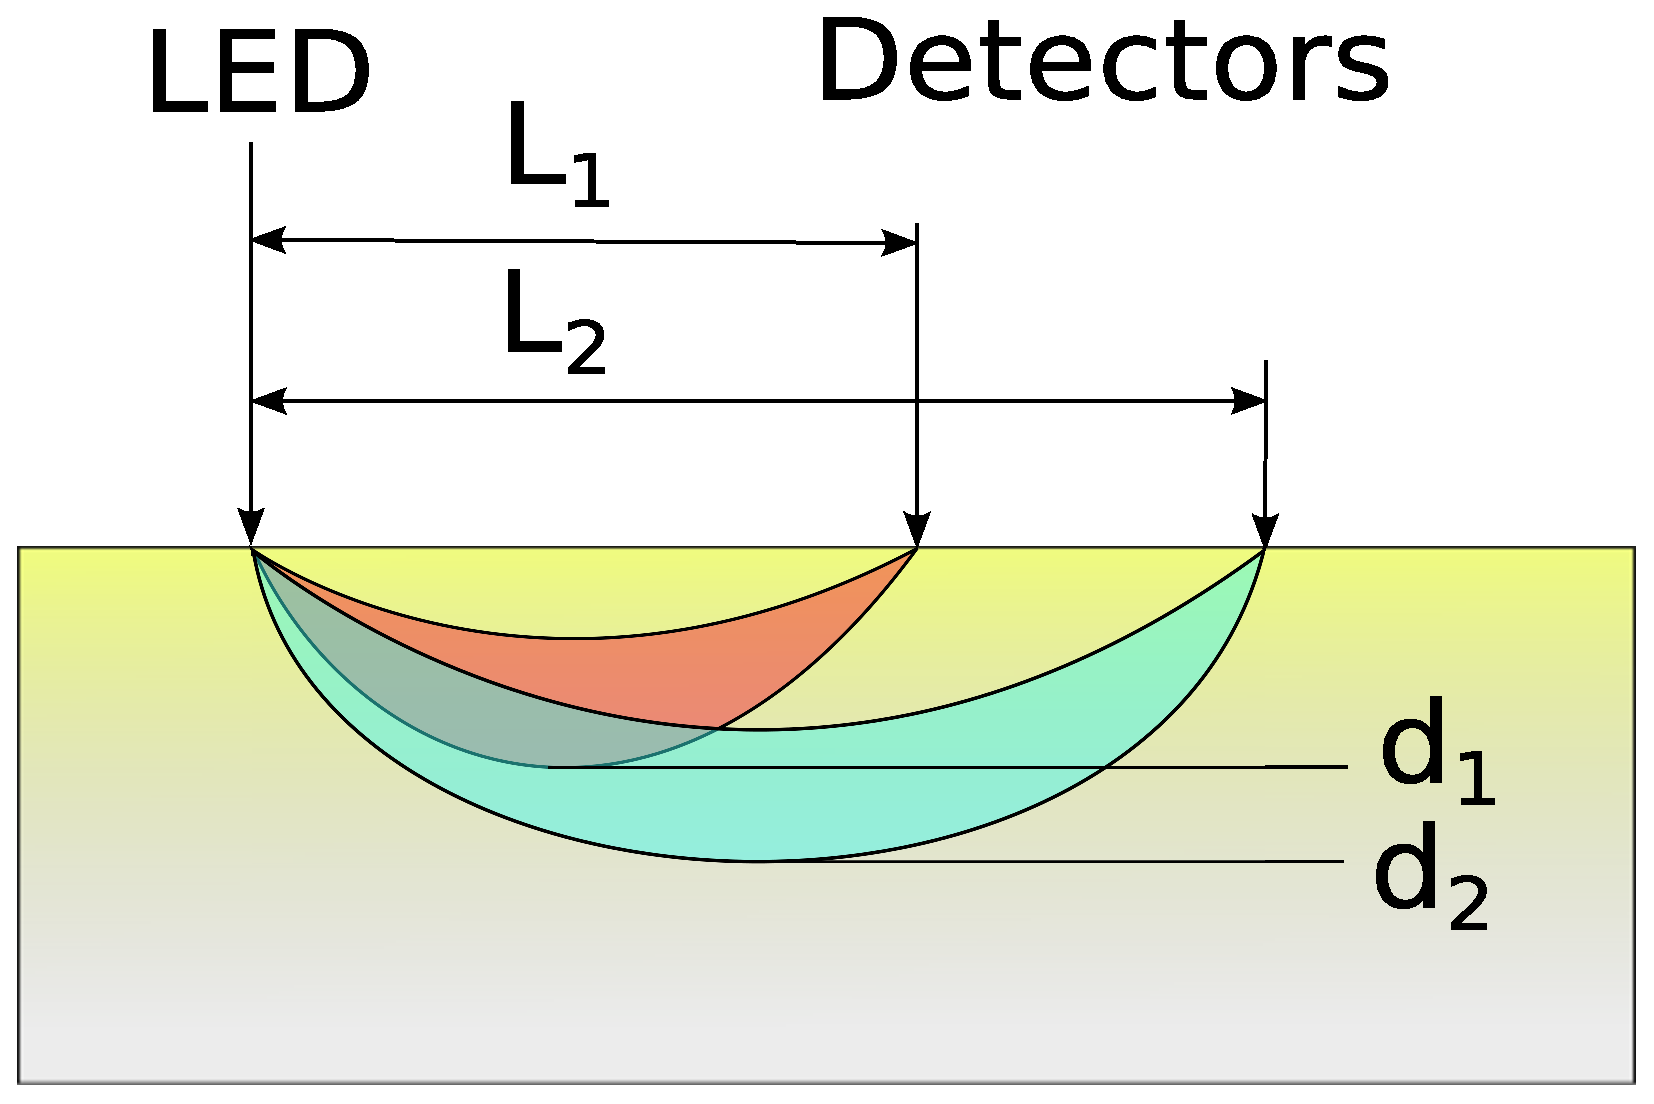
\includegraphics{fnir-penetration}
  \caption[Penetration by fNIR]{\label{fig:fnirpenetration}Penetration depth of a fNIR detector as a function of the distance between the NIR emitter and detector.  Light emitted by either an LED or fiber optic (red star) from the left passes through the tissue before it is scattered back to be detected (blue circle).  The path it takes through the tissue is determined by the distance between the emitter and detector.  A larger separation between emitter and detector (L$_2$) allows the light to penetrate deeper in to the tissue (d$_2$).  Modified after~\citep{head2010}}
\end{figure}

Three techniques are used to illuminate the tissue: (i)~time domain (or time resolved spectroscopy, TRS), (ii)~frequency domain and, (iii)~continuous wave illumination~\citep{izzetoglu2004}.  In TRS, short pulses of light are incident on the tissue and the temporal distribution of photons in measured.  In frequency domain spectroscopy, the amplitude of the incident light is modulated at a high frequency (10--100~MHz) and the phase shift and amplitude decay of the detected light is compared to the incident light~\citep{boas2002}. In continuous wave illumination, the incident light is not modulated so the detected light can only be compared for amplitude attenuation~\citep{izzetoglu2004}.

All of the techniques use the Beer-Lambert Law~\citep{beerlambert}
\begin{equation}
  I = I_0 e^{-\alpha (\lambda) x} \label{eq:beerlambert1}
\end{equation} 
modified to isolate the individual contributions from oxyHb and deoxyHb~\citep{cope}:
\begin{equation}
  \label{eq:modifiedbeerlamber}
  I = G I_0 e^{-(\alpha_{deoxyHb}C_{deoxyHb}+\alpha_{oxyHb}C_{oxyHb}) l} 
\end{equation}
where G is a factor to adjust for the measurement geometry, $I_0$ is in the incident light intensity, $\alpha_{oxyHb}$ and $\alpha_{deoxyHb}$ are the molar extinction coefficients for oxyHb and deoxyHb, $C_{oxyHb}$ and $C_{deoxyHb}$ are the chromophore concentrations for oxyHb and deoxyHb, and l is the path length~\citep{izzetoglu2004}.  By comparing a baseline measurement~($I_b$) with a new measurement~($I$), the optical density can be determined~\citep{izzetoglu2004}
\begin{equation}
  \Delta OD = \log \frac{I_b}{I} = \alpha_{deoxyHb} \Delta C_{deoxyHb}+\alpha_{oxyHb} \Delta C_{oxyHb}
\end{equation}
As discussed in~\citet{izzetoglu2004}, at least two wavelengths are utilized in the spectral window (700--1000~nm) in order to determine the change in concentration of chromophores $\Delta C_{deoxyHb}$ and $\Delta C_{oxyHb}$.  With these values, the oxygenation and total blood volume can be determined:
\begin{align}
  \label{eq:o2bloodvolume}
  Oxygenation\ &= \Delta C_{HBO2} - \Delta C_{HB} \nonumber \\
  Blood\ Volume\ &= \Delta C_{HBO2} + \Delta C_{HB} 
\end{align}
Using this method to experimentally measure the blood oxygenation while measuring the fMRI BOLD response could be used to refine the present model for calculating the metabolism and blood flow from the BOLD response.

While fNIRS does not provide spatially-precise measurements as fMRI, it should be possible to modify the existing model for calculating temperature from the BOLD response to use fNIR data. This would be advantageous because fNIRS systems are cheaper and less disruptive than fMRI systems, meaning they can be used with a wider range of patients (children and the elderly).  For this reason, developing a model which uses fNIRS data should be considered in future research.

\section{Thermal Imaging}
\label{sec:ThermalImaging}
The primary challenge in brain temperature research is performing brain temperature experimental measurements.  Since it is non-invasive, thermal imaging is appealing as a possible replacement for damaging thermocouple probes.  Unfortunately, this technique is limited by the high absorption of mid-infrared photons by water.

Light absorption by a material is modeled using the Beer-Lambert law
\begin{equation}
  I = I_0 e^{-\alpha (\lambda) x} \label{eq:beerlambert}
\end{equation}
where $I$ is the intensity at a depth $x$ remaining from light with an incident intensity $I_0$ in a material with absorption coefficient $\alpha$.  The point at which the intensity has decayed to 1/$e$ (about 37\%) of the incident intensity is called the penetration depth, $\delta_{p}$
\begin{equation}
  \delta_p = \frac{1}{\alpha (\lambda)} \label{eq:penetrationdepth}
\end{equation}
This equation can be used along with the black-body spectrum at tissue temperatures (\cref{fig:blackbody}) we can estimate the penetration depth of mid-infrared photons passing through water.

\begin{figure}[p]
  \centering
  $ 
	\begin{array}{c}
		\includegraphics[width=0.75\linewidth]{blackbody-1} \\
		\includegraphics[width=0.75\linewidth]{blackbody-2} 
	\end{array}
	$
  \caption[Black-body Spectrum at 250, 310 and 350 K]{\label{fig:blackbody}(a) Black-body spectrum at 250, 310 and 350 K calculated using Planck's Law. The black dashed line traces the peak in the spectrum as temperature changes.  As the temperature increases, differences in temperature translate to smaller shifts in peak wavelength compared to cooler temperatures. (b) A comparision of the black-body spectrum at 310 K and 310.025 K.  This is the shift in local temperature that would be expected under strong stimulation.}
\end{figure}
\begin{figure}[tb]
  \centering
  \includegraphics{water-wide-band}
  \caption[Wide-band absorption spectra of water]{\label{fig:waterabs}The absorptions spectra of water from UV to far-infrared.  Modified from~\citet{hale73}.}
\end{figure}

Wien's Displacement Law is a solution to Planck's law for the peak light emission wavelength:
\begin{align}
  \lambda_{max} &= \frac{b}{T} \label{eq:wienslaw} \\
  b &= 2.897\,7721 * 10^{-3} \mbox{ K m} \nonumber
\end{align}
where $b$ is Wien's displacement constant and T is the temperature in kelvin.  For $T=310$~K ($T=37\degree$~C), Wien's law yields a peak black-body emission wavelength of 9.347$\,$652~\textmu m. A physiologically reasonable temperature change to expect from stimulation is on the order of 0.01\degree C which corresponds to a new peak wavelength of 9.347$\,$350~\textmu m (T=310.01 K) or a shift of 0.302 nm.

The values of the absorption coefficient and the penetration depth of photons in water is shown in~\cref{fig:waterabs}. Looking at around 9.3~\textmu m, the absorption coefficient is approximately 700 cm$^{-1}$ which corresponds to a penetration depth of approximately 14~\textmu m.  This depth is roughly three orders of magnitude smaller than the distance from the surface of the brain to the surface of the head.  Further, all photons emitted as blackbody radiation (ranging from 3~\textmu m to over 30~\textmu m) have a penetration depth of less than 100 microns.  Thus, a thermal imaging camera is unable to image photons coming from the brain.

When thermal imaging is used, the photons collected come from the skin of the head rather than from any deeper tissues, thus it is not a viable form of brain activity detection unless direct line of sight to the brain is available (such as in an open skull surgery).  The noise-equivalent temperature difference (NETD) of currently available cameras is greater than 14~mK~\citep{flir,ici} or 7~mK~\citep{gunapala2002} for a camera which is not commercially available, so it would be limited to only the most extreme of excitations even if line of site to the brain is available.  As a comparison, the finger-tapping task discussed in the results section (\cref{sec:experimentalresults}) only induced a peak temperature change of 25~mK after tapping for about 170~seconds.  Detection of this activity would be at the limits of a thermal imaging camera.

While its applications to detecting brain activity are limited, thermal cameras could be useful in the operating room.  It has been found that inducing mild hypothermia in patients being treated for cerebral ischemia improves the clinical outcome~\citep{maher1993}. The same treatment has been shown to improve the outcome of patients who have experienced a stroke~\citep{krieger2001} and even in patients with severe head injuries~\citep{soukup2002}. The temperature of the brain is currently inferred from the core body temperature (which is monitored via an invasive thermistor catheter). If it is possible to directly image the brain (i.e. during surgery) then the hypothermia treatment can be better monitored through a thermal imaging camera.  This would be especially useful since conductive and radiative heat loss to the air from an exposed brain could reduce how tightly the brain temperature is regulated by the arterial blood temperature.  Since the tissue will be directly exposed to the surrounding air, \cref{eq:bioheat} would need to include a term for the radiative heat loss:
\begin{equation}
  C_{tissue} \frac{dT(t)}{dt} = ... +\frac{A \sigma T^4}{\rho_{gm} V}
\end{equation}
After rearranging to solve for $\frac{dT}{dt}$ and substituting values in, it is found that the change in temperature is approximately 0.07 K/s:
\begin{align}
  \frac{dT}{dt} &= \frac{A \sigma T^{4}}{\rho_{gm} V C_{tissue}}\nonumber\\
  & {} = \frac{1}{6}%
  \frac{%
    \left(6*4\ 10^{-6}\ \text{m}^{2}\right)%
    \left(5.6704\ 10^{-8}\ \frac{J}{\text{s m}^{2}\ \text{K}^{4}}\right)%
    \left(310\ \text{K}\right)^{4}}%
  { \left(1035\ 10^3\ \frac{\text{g}}{\text{m}^{3}}\right)%
    \left(8\ 10^{-9}\ \text{m}^3\right)%
    \left(3.664\ \frac{\text{J}}{\text{g K}}\right)}\nonumber\\
  & {} \approx 0.0690454\ \frac{\text{K}}{\text{s}}
\end{align}
where A and V are the surface area and volume of the voxel, $\sigma$ is the Stefan–Boltzmann constant and $\rho_{gm}$ is the density of gray matter.  The factor $1/6$ is there because only one face of the voxel is exposed to air.  Radiation passing through the other faces will be reabsorbed by the tissue~(\cref{fig:waterabs}).

Optical detectors face many challenges working with biological tissue, the worst being infrared light absorption by water. fNIRS works within an optical window in the water absorption in order to measure changes in blood oxygenation, while thermal imaging is limited to measuring the temperature of tissue it has direct line of sight with because of the high absorption of water in the operating window. Despite their limitations, both of these techniques could be used in future studies to improve our understanding of brain temperature dynamics.